% Don't touch this %%%%%%%%%%%%%%%%%%%%%%%%%%%%%%%%%%%%%%%%%%%
\documentclass[addpoints]{exam}
\usepackage{fullpage}
\usepackage[left=1.0in,top=1.0in,right=1.0in,bottom=1.0in,headheight=3ex,headsep=3ex]{geometry}
\usepackage{graphicx}
\usepackage{float}
\usepackage{adjustbox}
\usepackage{comment}
\usepackage{tikz}
\usetikzlibrary{calc}
\usetikzlibrary{matrix}
\usetikzlibrary{positioning}
\usepackage{amsmath}

\tikzset{   
	every picture/.style={remember picture,baseline},
	every node/.style={anchor=base,align=center,outer sep=1.5pt},
	every path/.style={thick},
}
\newcommand\marktopleft[1]{%
	\tikz[overlay,remember picture] 
	\node (marker-#1-a) at (-.3em,.3em) {};%
}
\newcommand\markbottomright[2]{%
	\tikz[overlay,remember picture] 
	\node (marker-#1-b) at (0em,0em) {};%
}
\tikzstyle{every picture}+=[remember picture] 
\tikzstyle{mybox} =[draw=black, very thick, rectangle, inner sep=10pt, inner ysep=20pt]
\tikzstyle{fancytitle} =[draw=black,fill=red, text=white]


\usepackage{graphicx,stackengine,xcolor}
\newcommand\Circle[1]{%
	\def\useanchorwidth{T}%
	\def\stacktype{L}%
	\stackon[0pt]{#1}{\scalebox{2.0}[1.15]{\textcolor{red}{$\bigcirc$}}}%
}
\newcommand{\blankline}{\quad\pagebreak[2]}
%%%%%%%%%%%%%%%%%%%%%%%%%%%%%%%%%%%%%%%%%%%%%%%%%%%%%%%%%%%%%%

% Modify Course title, instructor name, semester here %%%%%%%%

\title{ECN 453: Mid-term Exam 1}
% Modify header here %%%%%%%%%%%%%%%%%%%%%%%%%%%%%%%%%%%%%%%%%
\rhead{\footnotesize ECN 453: Mid-term Exam 1}

\date{} 

\begin{document}
	\maketitle
	\begin{center}
		\fbox{\fbox{\parbox{6in}{\centering\
					\textbf{Instructions}:
					\begin{itemize}
					\item You have \textbf{70 minutes}
					\item Please write your final answer in the underlined section provided. 
					\item You may bring a calculator and notes on a two-sided cheat-sheet on letter-size paper. 
					\item Please be neat. If your work is too messy it will not be graded.
					\item Be sure to show your working.
					\item This is a long exam, so there are lots of ways to get points. If you get stuck, move on!
					\item Good luck!
					\end{itemize}	
			}}}
	\end{center}
	
	\vspace{5mm}
	\makebox[0.75\textwidth]{Name: \enspace\hrulefill}
	\vspace{50pt}
	\begin{center}
		\gradetable[h][questions]
	\end{center}
	
	\newpage
	
\begin{questions}
	\subsection*{Short Answer Questions (30 points)}
	\vspace{11pt}
	\question Depending on the question, write either: 
	\begin{itemize}
		\item a number 
		\item one of: True, False, or NEI (Not Enough Information)
		\item a definition (i.e. one or a few words)
	\end{itemize}
	\vspace{11pt}
	\begin{parts}
		\part[3] A monopolist faces the constant elasticity demand curve $p=7q^{1/-2}$ and has a constant marginal cost = 2. What is the optimal price?
		
		\answerline[answer]
		
		\part[3] The \textit{centipede game} that we discussed in class is often used as an example of a game that violates \textit{which assumption} when played in real-world experimental settings?
		
		\answerline[answer]
		
		\part[3] Suppose that a monopolist has the cost $C(q)= 10+2q^2$ and the perfect competition price and quantity is at $p_{pc} = 8, q_{pc} = 2$. What subsidy will the regulator need to provide the monopolist to ensure it does not shutdown under \textit{marginal cost pricing}?
		
		\answerline[answer]
		
		\part[3] True, False, or Not Enough Information: dead-weight-loss is always eliminated by average-cost pricing.
		
		\answerline[answer]
		
		\part[3] True, False, or Not Enough Information: if there is a dominated strategy in a game with two players and two strategies per player, then there is \textit{always} a dominant strategy.
		
		\answerline[answer]
		
		\part[3] True, False, or Not Enough Information: consumer surplus always decreases when moving from uniform pricing to price discrimination.
		\answerline[answer]
		
		\part[3] A monopolist faces a constant price elasticity demand curve, has a constant marginal cost of 2, and is optimally setting a price of 5. What is the price elasticity of demand?
		
		\answerline[answer]
		
		
		\part[3] In the case \textit{FTC vs. Facebook} that we discussed in class, the FTC is seeking \textit{what remedy} to Facebook's ownership of Instagram and Whatsapp?
		
		\answerline[answer]
		
		\part[3] True, False, or Not Enough Information: given two markets, a monopolist will charge a higher \textit{price-cost margin} in a market with more elastic demand. 
		
		\answerline[answer]
		
		\part[3] True, False, or Not Enough Information: dead-weight-loss is zero under perfect price discrimination.
		
		\answerline[answer]
		

	\end{parts}
	
	\subsection*{Movie Theater Question (30 points)}
	\question Suppose you are the owner of a movie theater. There are two types of customers: students (denoted `s') and non-students (denoted `ns'). The demand for movie seats for each of these segments is:
	\begin{align*}
		\text{Student: } &q_{s} = 70 - 2p_{s} \\
		\text{Non-student: }& q_{ns} = 80 - p_{ns}
	\end{align*}
	\begin{parts}
		\part [20] Assume that you cannot distinguish between students and non-students, and so you can only set a single \textit{uniform price} for all consumers. Assume that the marginal cost of a seat is \$16. What is the optimal uniform price? (Hint: plot marginal revenue.) 
		\vspace{500pt}
		\answerline[answer] 
		\newpage
		\part[10] Suppose that there are only (identical) students in the market, and that the interpretation of the demand curve for students is now \textit{how many} tickets each student demands. Assume that the marginal cost of a seat is \$2.
		
		You would like to offer a `movie-pass' plan where each customer pays a fixed fee and then can watch as many movies as they want (i.e. at a variable price = 0). What is the optimal fixed fee for the movie-pass plan?
					\vspace{500pt}
		\answerline[answer] 
	\end{parts}
	\newpage
	\subsection*{Price Discrimination By Self-Selection (30 points)}
\question Suppose you are the CEO of an airline and there are two segments of airline ticket consumers: business and tourists. \underline{Marginal cost = \$20 per seat.} 

There are two types of tickets: standard and restricted, where a restricted ticket has limitations about when/where it can be used (and so we can think of it as a `damaged' good). The number of consumers and willingness-to-pay for each consumer is given in the following table:

\begin{centering}
	\begin{table}[h]
		\centering
		\begin{tabular}{|l|c|c|c|}
			\hline
			\textbf{Consumer type}&  \textbf{Number of consumers} & \multicolumn{2}{c}{\textbf{Willingness to pay (\$)}} \\
			%\hline
			& & Standard & Restricted  \\
			\hline
			Business & 10 & 135 & 70  \\
			\hline
			Tourist & 40  & 60 & 40  \\
			\hline
		\end{tabular}
	\end{table}
\end{centering}
\begin{parts}
	\part[5] What is the profit under perfect price discrimination?
	\vspace{200pt}
	\answerline[answer] 
	\part Assume that you \underline{cannot} distinguish between business and tourist consumers.
	\begin{subparts}
		\subpart[10] If you can only offer the standard ticket, what is the optimal uniform price?
			\vspace{200pt}
		\answerline[answer] 
		\newpage
		\subpart[10] Suppose that you offer both tickets and charge $\$40$ for the restricted ticket. What is the optimal price for the standard ticket?
			\vspace{250pt}
		\answerline[answer] 
		\subpart[5] Suppose that you offer both tickets and charge $\$80$ for the restricted ticket. What is the optimal price for the standard ticket?
					\vspace{250pt}
		\answerline[answer] 
	\end{subparts}
\end{parts}

\newpage
\subsection*{Game Theory: Entry Deterrence (30 points)}
\question Consider the following game with two players: an Entrant and an Incumbent. The strategies of the Entrant are to enter `E' or don't enter `DE'. The strategies of the Incumbent are to retaliate `R' or don't retaliate `DR'. In the payoffs, `x' represents a number.

\begin{figure}[h]
	\centering
	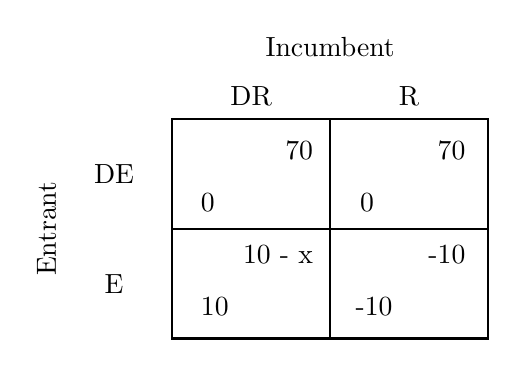
\begin{tikzpicture}
		\matrix[matrix of math nodes,every odd row/.style={align=right},every evenrow/.style={align=left},every node/.style={text width=1.5cm},row sep=0.2cm,column sep=0.2cm,ampersand replacement=\&] (m) {
			70 \& 70 \\
			0 \phantom{---------} \& 0 \phantom{--------} \\
			10 - x \& -10\\
			10 \phantom{--------} \& -10 \phantom{------}  \\
		};
		\draw (m.north east) rectangle (m.south west);
		\draw (m.north) -- (m.south);
		\draw (m.east) -- (m.west);
		
		% Player 1
		\coordinate (c) at ($(m.north west)!0.25!(m.south west)$);
		\coordinate (d) at ($(m.north west)!0.75!(m.south west)$);
		\node[left=2pt of c,text width=1cm]  {DE};
		\node[left=2pt of d,text width=1cm]  {E};
		
		% Player 2
		\coordinate (a) at ($(m.north west)!0.25!(m.north east)$);
		\coordinate (b) at ($(m.north west)!0.75!(m.north east)$);
		\node[above=5pt of a,anchor=base] {DR};
		\node[above=5pt of b,anchor=base] {R};
		
		\node[above=18pt of m.north] (firm b) {Incumbent};
		\node[left=1.6cm of m.west,rotate=90,align=center,anchor=center] {Entrant};
		
		%\node[above=5pt of firm b]  {Payoff Matrix};
	\end{tikzpicture}
\end{figure}

\begin{parts}
	\part[5] Assume that $x=0$. What are all the Nash equilibria?
				\vspace{400pt}
	\answerline[answer] 
	\newpage
	\part[10] Assume that $x=0$ and that the players play $(E, DR)$ in the simultaneous game. What is the maximum value that the Incumbent would pay to commit to moving first?
				\vspace{600pt}
	\answerline[answer] 
	\newpage
	\part[15] Assume that the Entrant moves first. What values of $x$ successfully deter entry (i.e. ensure that in the subgame-perfect equilibrium, the Entrant plays DE)?
				\vspace{600pt}
	\answerline[answer] 
\end{parts}

\end{questions}


\end{document}